\documentclass{article}
\usepackage[main=spanish, provide=*]{babel}
\usepackage{xcolor}
\usepackage{sansmath}
\usepackage{array}
\usepackage{graphicx}
\usepackage{tikz}
\usepackage{circuitikz}
\usepackage{pgfplots}
\usepackage{darkmode}
\usepackage{amsmath}
\usepackage{svg}
\usepackage[a4paper, top=2cm, bottom=2cm]{geometry}

\sansmath
\renewcommand{\rmdefault}{cmss}

\newcommand{\iconpath}{/home/khz/git/tabler-icons/icons/outline-white/}
\newcommand{\icon}[1]{\includesvg[width=0.75em]{\iconpath#1}}
\newcommand{\instrumentopath}{/home/khz/Documentos/Carrera/MusiKe/instrumentos/svg/}
\newcommand{\instrumento}[1]{\raisebox{-0.6em}{\includesvg[width=2em]{\instrumentopath#1}}}

\enabledarkmode

\definecolor{c1}{HTML}{8bb6e7}
\definecolor{c2}{HTML}{87f3dd}
\definecolor{c3}{HTML}{fdef83}
\definecolor{c4}{HTML}{fdc373}
\definecolor{c5}{HTML}{fd8581}
\definecolor{c6}{HTML}{c573e7}
\definecolor{c7}{HTML}{afdb68}
\definecolor{c8}{HTML}{e59f8b}

\definecolor{page}{HTML}{262626}
\pagecolor{page}

\begin{document}
\title{MusiKe}
\author{Mario López Sáez}
\date{\today}
\maketitle

\begin{center}
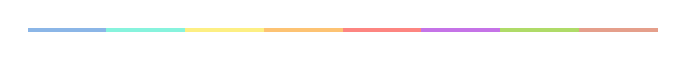
\begin{tikzpicture}
    \fill[c1] (0, 0) rectangle ++(1, 0.05);
    \fill[c2] (1, 0) rectangle ++(1, 0.05);
    \fill[c3] (2, 0) rectangle ++(1, 0.05);
    \fill[c4] (3, 0) rectangle ++(1, 0.05);
    \fill[c5] (4, 0) rectangle ++(1, 0.05);
    \fill[c6] (5, 0) rectangle ++(1, 0.05);
    \fill[c7] (6, 0) rectangle ++(1, 0.05);
    \fill[c8] (7, 0) rectangle ++(1, 0.05);
\end{tikzpicture}

\end{center}

\tableofcontents
\newpage



\section{Descripción del Proyecto}

MusiKe es un juego educativo e interactivo diseñado para que usuarios de todas las edades descubran y aprendan los instrumentos de la orquesta a través de divertidos retos y minijuegos. La aplicación está desarrollada para Android usando Java y la librería AppCompat.

\section{Estructura del Proyecto}

\begin{itemize}
  \item \icon{folder} \textbf{app/src/main/java/mario/khz/musike}: contiene las actividades y clases principales de la aplicación.
  \item \icon{photo-scan} \textbf{app/src/main/res/drawable}: recursos gráficos vectoriales (iconos de instrumentos, fondos y botones).
  \item \icon{volume-2} \textbf{app/src/main/res/raw}: archivos de audio con sonidos de los instrumentos de la orquesta.
  \item \icon{file-text} \textbf{README.md}: descripción general del proyecto y logo.
  \item \icon{file} \textbf{tex/MusiKe.tex}: este documento de documentación.
\end{itemize}


\section{Assets}

\subsection{Instrumentos \icon{music}}

A continuación se listan los instrumentos incluidos en la aplicación, junto a sus recursos gráficos y de audio:

\begin{itemize}
  \item \instrumento{viola} Violín: \texttt{res/drawable/violin.xml}, \texttt{res/raw/violin.mp3}
  \item \instrumento{viola} Viola: \texttt{res/drawable/viola.xml}, \texttt{res/raw/viola.mp3}
  \item \instrumento{cello} Violonchelo: \texttt{res/drawable/cello.xml}, \texttt{res/raw/cello.mp3}
  \item \instrumento{contrabajo} Contrabajo: \texttt{res/drawable/contrabajo.xml}, \texttt{res/raw/contrabajo.mp3}
  \item \instrumento{piano} Piano: \texttt{res/drawable/piano.xml}, \texttt{res/raw/piano.mp3}
  \item \instrumento{flauta} Flauta: \texttt{res/drawable/flauta.xml}, \texttt{res/raw/flauta.mp3}
  \item \instrumento{oboe} Oboe: \texttt{res/drawable/oboe.xml}, \texttt{res/raw/oboe.mp3}
  \item \instrumento{clarinete} Clarinete: \texttt{res/drawable/clarinete.xml}, \texttt{res/raw/clarinete.mp3}
  \item \instrumento{fagot} Fagot: \texttt{res/drawable/fagot.xml}, \texttt{res/raw/fagot.mp3}
  \item \instrumento{trompeta} Trompeta: \texttt{res/drawable/trompeta.xml}, \texttt{res/raw/trompeta.mp3}
  \item \instrumento{trombon} Trombón: \texttt{res/drawable/trombon.xml}, \texttt{res/raw/trombon.mp3}
  \item \instrumento{trompa} Trompa: \texttt{res/drawable/trompa.xml}, \texttt{res/raw/trompa.mp3}
  \item \instrumento{tuba} Tuba: \texttt{res/drawable/tuba.xml}, \texttt{res/raw/tuba.mp3}
  \item \instrumento{arpa} Arpa: \texttt{res/drawable/arpa.xml}, \texttt{res/raw/arpa.mp3}
  \item \instrumento{marimba} Marimba: \texttt{res/drawable/marimba.xml}, \texttt{res/raw/marimba.mp3}
  \item \instrumento{vibrafono} Vibráfono: \texttt{res/drawable/vibrafono.xml}, \texttt{res/raw/vibrafono.mp3}
  \item \instrumento{pequena_percusion} Pequeña percusión: \texttt{res/drawable/pequena\_percusion.xml}, \texttt{res/raw/pequena\_percusion.mp3}
  \item \instrumento{platos_de_choque} Platos de choque: \texttt{res/drawable/platos\_de\_choque.xml}, \texttt{res/raw/platos\_de\_choque.mp3}
  \item \instrumento{campanologo} Campanólogo: \texttt{res/drawable/campanologo.xml}, \texttt{res/raw/campanologo.mp3}
  \item \instrumento{caja} Caja: \texttt{res/drawable/caja.xml}, \texttt{res/raw/caja.mp3}
\end{itemize}
\subsection{Iconos de Instrumentos}

Los iconos de los instrumentos han sido obtenidos de \texttt{https://www.freepik.com/} y procesados posteriormente con el siguiente código:

\begin{figure}[h]
\centering
\includegraphics[width=\textwidth]{svg_codigo.png}
\caption{Código de procesamiento de SVG.}
\end{figure}

\subsection{Audios de Instrumentos}

Los audios han sido obtenidos de un CD que me ha prestado un profesor de Música para la realización de este proyecto.

\subsection{Otros Recursos Gráficos \icon{photo-scan}}
Además de los iconos de los instrumentos, la aplicación utiliza otros recursos gráficos para construir una interfaz de usuario coherente y atractiva:
\begin{itemize}
    \item \textbf{Fondos con degradado}: Las pantallas principales de la aplicación utilizan fondos con un suave degradado diagonal. Estos se definen en \texttt{res/drawable/} como ficheros XML de tipo \texttt{<shape>}, lo que permite una representación eficiente y escalable sin necesidad de imágenes de mapa de bits.
    \item \textbf{Botones redondeados}: Todos los botones interactivos presentan esquinas redondeadas para una estética moderna y amigable. Al igual que los fondos, se definen mediante XML de tipo \texttt{<shape>}, especificando el radio de las esquinas (\texttt{<corners>}) y el color de fondo.
    \item \textbf{Iconos de la interfaz}: Para mejorar la navegación y la comprensión visual, se utilizan iconos vectoriales en varios puntos de la aplicación (ej: en los botones del menú principal). Estos iconos provienen de la librería de código abierto \textit{Tabler Icons} (también en este documento) y están integrados como \texttt{VectorDrawable} en formato XML, garantizando una visualización nítida en cualquier densidad de pantalla.
\end{itemize}


\section{Activities}

La arquitectura de la aplicación se articula en torno a un conjunto de Activities, cada una responsable de una pantalla y una funcionalidad concreta. A continuación, se detalla el propósito y funcionamiento de cada una de ellas.

\subsection{MainActivity \icon{layout-dashboard}}
Es la actividad principal y el punto de entrada de la aplicación. Su función es presentar al usuario la pantalla de bienvenida y actuar como un distribuidor central, ofreciendo las dos modalidades principales de la aplicación:
\begin{itemize}
    \item \textbf{Modo Estudio}: Inicia \texttt{StudyActivity} para el aprendizaje libre.
    \item \textbf{Modo Juego}: Lanza \texttt{RoundSelectionActivity} para comenzar una partida.
\end{itemize}

\subsection{StudyActivity \icon{book}}
Esta actividad está diseñada para el aprendizaje y la consulta. Proporciona una interfaz donde el usuario puede explorar los instrumentos de la orquesta. Al seleccionar un instrumento, la actividad reproduce su sonido característico, permitiendo una familiarización auditiva y visual sin la presión de un entorno de juego.

Para la presentación visual de los instrumentos, esta actividad utiliza un componente auxiliar llamado \texttt{StudyGridAdapter}, que se encarga de:
\begin{itemize}
    \item \textbf{Estructurar la cuadrícula}: Organiza los instrumentos en una rejilla de 4 columnas mediante un \texttt{GridLayout}.
    \item \textbf{Crear celdas interactivas}: Genera para cada instrumento un contenedor con un botón de imagen que muestra el icono vectorial del instrumento y una etiqueta con su nombre.
    \item \textbf{Gestionar la reproducción}: Implementa los listeners que reproducen el sonido correspondiente cuando el usuario pulsa sobre un instrumento.
\end{itemize}

\subsection{RoundSelectionActivity \icon{list}}
Actúa como una antesala al modo de juego. Su único propósito es permitir al usuario configurar la partida, seleccionando el número de rondas que desea jugar. Una vez que el usuario ha hecho su elección, esta actividad inicia la \texttt{GameActivity}, pasándole la configuración seleccionada como un \textit{extra} en el \texttt{Intent}.

\subsection{GameActivity \icon{device-gamepad-2}}
Es el núcleo interactivo de MusiKe. Esta actividad gestiona la lógica del juego de identificación de instrumentos, que se desarrolla de la siguiente manera:
\begin{itemize}
    \item \textbf{Inicio y carga}: Al comenzar, lee el fichero \texttt{assets/instruments.json} para cargar la información de los instrumentos. A continuación, baraja la lista para crear un orden aleatorio de preguntas para la partida.
    \item \textbf{Desarrollo de la ronda}: En cada ronda, reproduce el sonido de un instrumento y presenta al usuario cuatro botones con nombres de instrumentos como posibles respuestas. Para aumentar el desafío, las opciones incorrectas se eligen preferentemente de la misma familia que la respuesta correcta.
    \item \textbf{Interacción y feedback}: El usuario selecciona una opción. La aplicación le proporciona feedback visual inmediato (verde para acierto, rojo para error). Si falla, se le indica cuál era la respuesta correcta. Tras una breve pausa, la actividad avanza automáticamente a la siguiente ronda.
    \item \textbf{Finalización}: Una vez completadas todas las rondas, \texttt{GameActivity} recopila las estadísticas de la partida (número de aciertos, respuestas del usuario y respuestas correctas) y lanza la \texttt{FinishActivity} para mostrar los resultados.
\end{itemize}

\subsection{FinishActivity \icon{award}}
Esta es la pantalla final del ciclo de juego. Su objetivo es mostrar al usuario un resumen de su rendimiento en la partida. Presenta la puntuación final (ej: "8 de 10 aciertos") y una tabla detallada que muestra las respuestas correctas para cada ronda, reforzando así el aprendizaje.

\subsection{CircleProgressView \icon{chart-pie}}
Aunque no es una Activity, es un componente de interfaz de usuario (View) personalizado de vital importancia en \texttt{GameActivity}. Su función es mostrar una barra de progreso circular que se actualiza en tiempo real, sincronizada con la reproducción del audio del instrumento. Esto proporciona al usuario una referencia visual clara de la duración del sonido y del tiempo restante para responder, mejorando significativamente la experiencia de juego.

\section{Aspectos Técnicos}

En esta sección se abordan decisiones de implementación y detalles técnicos clave que definen la robustez y escalabilidad de la aplicación.

\subsection{Vinculación de Recursos y Datos}
Se ha adoptado una estrategia de nomenclatura unificada para los recursos. Cada instrumento definido en \texttt{assets/instruments.json} tiene un campo \texttt{file} (ej: \texttt{"violin"}) que actúa como identificador único. Este identificador se corresponde directamente con el nombre de los ficheros de recursos asociados:
\begin{itemize}
    \item \textbf{Recurso gráfico}: \texttt{res/drawable/violin.xml}
    \item \textbf{Recurso de audio}: \texttt{res/raw/violin.mp3}
\end{itemize}
Esta convención permite cargar dinámicamente los recursos en el código Java mediante \\
\texttt{getResources().getIdentifier()}, simplificando enormemente la gestión y la adición de nuevos instrumentos, ya que no es necesario modificar el código para vincular los nuevos assets.

\subsection{Evolución de la Lógica del Juego}
La mecánica de selección de preguntas en \texttt{GameActivity} ha pasado por una mejora significativa:
\begin{itemize}
    \item \textbf{Implementación inicial}: En una primera fase, en cada ronda se seleccionaba un instrumento de forma completamente aleatoria de la lista total. Este enfoque, aunque sencillo, permitía que un mismo instrumento pudiera aparecer varias veces en una misma partida, resultando en una experiencia de juego repetitiva.
    \item \textbf{Implementación final}: Para solucionar esto, se implementó el método \texttt{generarOrdenRondas()}. Al inicio de cada partida, este método crea una lista con todos los instrumentos, la baraja de forma aleatoria y la almacena. Las rondas posteriores consumen instrumentos de esta lista pre-barajada, garantizando que cada instrumento aparezca como máximo una vez por partida, lo que resulta en una experiencia más variada.
\end{itemize}

\subsection{Gestión de la Interfaz y el Estado}
La aplicación gestiona el estado y la interfaz de usuario de manera eficiente:
\begin{itemize}
    \item \textbf{Paso de datos}: La comunicación entre Activities se realiza a través de \texttt{Intent extras}, un mecanismo estándar en Android para pasar datos como el número de rondas o los resultados finales.
    \item \textbf{Actualización en tiempo real}: El progreso de la reproducción de audio se visualiza en el \texttt{CircleProgressView} gracias a un \texttt{Handler} que actualiza la interfaz en segundo plano a intervalos regulares, proporcionando una respuesta visual fluida y sin bloquear el hilo principal.
    \item \textbf{Liberación de recursos}: En el método \texttt{onDestroy()} de la actividad, se liberan explícitamente los recursos del \texttt{MediaPlayer} y se detienen las actualizaciones del \texttt{Handler}. Esta práctica es fundamental para evitar fugas de memoria (\textit{memory leaks}) y asegurar el buen rendimiento de la aplicación.
\end{itemize}

\subsection{Gestión de la Orientación de Pantalla}
Se ha tomado una decisión estratégica respecto a la rotación de pantalla para optimizar la experiencia de usuario y la eficiencia del desarrollo:
\begin{itemize}
    \item \textbf{Bloqueo general a modo retrato}: La mayoría de las actividades de la aplicación, incluyendo \texttt{GameActivity}, están configuradas para funcionar exclusivamente en orientación vertical (retrato).
    \item \textbf{Excepción de StudyActivity}: La única excepción es la \texttt{StudyActivity}, que permite la rotación. Su diseño, basado en un \textit{ScrollView}, se adapta de forma natural a la orientación apaisada sin perjudicar la usabilidad.
    \item \textbf{Prevención de reinicio en GameActivity}: La razón principal para bloquear la rotación en la \texttt{GameActivity} es evitar el reinicio del ciclo de vida de la actividad que ocurre por defecto en Android al girar el dispositivo. Dicho reinicio provocaría la pérdida completa del estado de la partida (rondas, puntuación, etc.). Implementar la lógica para guardar y restaurar este estado (mediante \texttt{onSaveInstanceState}) habría añadido una complejidad considerable al desarrollo. Por tanto, forzar la orientación vertical se consideró una solución más pragmática y robusta para garantizar la continuidad del juego.
\end{itemize}

\end{document}
